%
% positiv.tex
%
% (c) 2021 Prof Dr Andreas Müller, OST Ostschweizer Fachhochschule
%
\section{Positive Vektoren und Matrizen
\label{buch:section:positive-vektoren-und-matrizen}}
\rhead{Positive Vektoren und Matrizen}
Die Google-Matrix und die Matrizen, die wir in Markov-Ketten angetroffen
\index{Google-Matrix}%
haben, zeichnen sich dadurch aus, dass alle ihre Einträge positiv oder
mindestens nicht negativ sind.
Die Perron-Frobenius-Theorie, die in diesem Abschnitt entwickelt
\index{Perron-Frobenius-Theorie}%
werden soll, zeigt, dass Positivität einer Matrix nützliche
Konsequenzen für Eigenwerte und Eigenvektoren hat.
Das wichtigste Resultat ist die Tatsache, dass positive Matrizen immer
einen einzigen einfachen Eigenwert mit Betrag $\varrho(A)$ haben,
was zum Beispiel die Konvergenz des PageRank-Algorithmus garantiert.
Dies wird im Satz~\ref{buch:wahrscheinlichkeit:satz:perron-frobenius}
von Perron-Frobenius in
Abschnitt~\ref{buch:subsection:der-satz-von-perron-frobenius}
erklärt.

%
% Elementare Definitionen und Eigenschaften 
%
\subsection{Elementare Eigenschaften
\label{buch:subsection:elementare-eigenschaften}}
In diesem Abschnitt betrachten wir ausschliesslich reelle Vektoren
und Matrizen.
Die Komponenten sind somit immer miteinander vergleichbar, daraus
lässt sich auch eine Vergleichsrelation zwischen Vektoren
ableiten.

\begin{definition}
Ein Vektor $v\in\mathbb{R}^n$ heisst {\em positiv}, geschrieben
$v>0$, wenn alle seine Komponenten positiv sind: $v_i>0\,\forall i$.
Ein Vektor $v\in\mathbb{R}^n$ heisst {\em nichtnegativ}, in Formeln
$v\ge 0$, wenn alle
seine Komponenten nicht negativ sind: $v_i\ge 0\,\forall i$.
\index{positiver Vektor}%
\index{nichtnegativer Vektor}%
\end{definition}

Geometrisch kann man sich die Menge der positven Vektoren in zwei Dimensionen
als die Punkte des ersten Quadranten oder in drei Dimensionen als die
\index{Quadrant}%
\index{Oktant}%
Vektoren im ersten Oktanten vorstellen.

Aus der Positivität eines Vektors lässt sich jetzt eine Vergleichsrelation
für beliebige Vektoren ableiten.
Mit der folgenden Definition wird erreicht, das mit Ungleichungen für Vektoren
auf die gleiche Art und Weise gerechnet werden kann, wie man sich
dies von Ungleichungen zwischen Zahlen gewohnt ist.

\begin{definition}
Für zwei Vektoren $u,v\in\mathbb{R}^n$ ist genau dann $u>v$, wenn
$u-v > 0$ ist.
Ebenso ist $u\ge v$ genau dann, wenn $u-v\ge 0$.
\end{definition}

Ungleichungen zwischen Vektoren kann man daher auch so interpretieren,
dass sie für jede Komponente einzeln gelten müssen.
Die Definition funktionieren analog auch für Matrizen:

\begin{definition}
Eine Matrix $A\in M_{m\times n}(\mathbb{R})$  heisst {\em positiv},
wenn alle ihre Einträge $a_{i\!j}$ positiv sind: $a_{i\!j}>0\,\forall i,j$.
Eine Matrix $A\in M_{m\times n}(\mathbb{R})$  heisst {\em nichtnegativ},
wenn alle ihre Einträge $a_{i\!j}$ nichtnegativ sind: $a_{i\!j}\ge 0\,\forall i,j$.
\index{positive Matrix}%
\index{nichtnegative Matrix}%
Man schreibt $A>B$ bzw.~$A\ge B$ wenn $A-B>0$ bzw.~$A-B\ge 0$.
\end{definition}

Die Permutationsmatrizen sind Beispiele von nichtnegativen Matrizen,
deren Produkte wieder nichtnegativ sind.
Dies ist aber ein sehr spezieller Fall, wie das folgende Beispiel
zeigt.

\begin{beispiel}
Wir betrachten die Matrix
\begin{equation}
A=
\begin{pmatrix}
0.9&0.1&   &   &   &   \\
0.1&0.8&0.1&   &   &   \\
   &0.1&0.8&0.1&   &   \\
   &   &0.1&0.8&0.1&   \\
   &   &   &0.1&0.8&0.1\\
   &   &   &   &0.1&0.9
\end{pmatrix}
\label{buch:wahrscheinlichkeit:eqn:diffusion}
\end{equation}
Die Multiplikation eines Vektors mit dieser Matrix bewirkt, dass die
Komponenten des Vektors auf benachbarte Komponenten ``verschmiert'' werden.
Wendet man $A$ wiederholt auf den ersten Standardbasisvektor $v_1=e_1$ an,
erhält man nacheinander die Vektoren $v_2=Av_1$, $v_n = Av_{n-1}$.
\begin{figure}
\centering
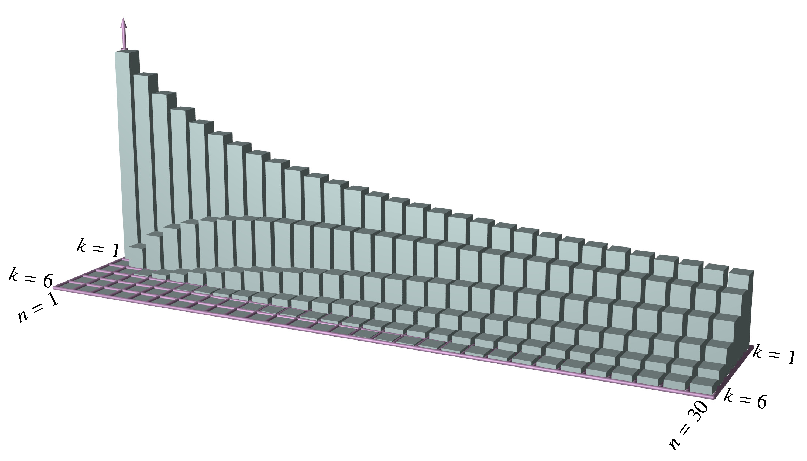
\includegraphics{chapters/80-wahrscheinlichkeit/images/diffusion.pdf}
\caption{Die sechs Komponenten für $k=1$ bis $k=6$ der Vektoren $A^{n-1}e_1$
für die Matrix $A$ in \eqref{buch:wahrscheinlichkeit:eqn:diffusion}
sind als Säulen dargestellt.
Sie zeigen, dass für genügend grosses $n$, alle Komponenten
des Vektors $A^{n-1}e_1$ positiv werden.
\label{buch:wahrscheinlichkeit:fig:diffusion}}
\end{figure}
In Abbildung~\ref{buch:wahrscheinlichkeit:fig:diffusion} sind die Komponenten
als Säulen dargestellt.
Man kann erkennen, dass für genügend grosse $n$ alle Komponenten
der Vektoren positiv werden.

Man kann auch direkt die Potenzen $A^n$ ausrechen und sehen, dass
\[
A^5
=
\begin{pmatrix}
   0.65658&  0.27690&  0.05925&  0.00685&  0.00041&  0.00001\\
   0.27690&  0.43893&  0.22450&  0.05281&  0.00645&  0.00041\\
   0.05925&  0.22450&  0.43249&  0.22410&  0.05281&  0.00685\\
   0.00685&  0.05281&  0.22410&  0.43249&  0.22450&  0.05925\\
   0.00041&  0.00645&  0.05281&  0.22450&  0.43893&  0.27690\\
   0.00001&  0.00041&  0.00685&  0.05925&  0.27690&  0.65658
\end{pmatrix}
>0
\]
und dass daher für alle $n\ge 5$ die Matrix $A^n$ positiv ist.
\end{beispiel}

Die Eigenschaft der Matrix $A$ von
\eqref{buch:wahrscheinlichkeit:eqn:diffusion}, dass $A^n>0$
für genügend grosses $n$ ist, ist bei Permutationsmatrizen nicht
vorhanden.
Die Zyklen-Zerlegung einer Permutationsmatrix zeigt, welche
Unterräume von $\mathbb{R}^n$ die iterierten Bilder eines
Standardbasisvektors aufspannen.
Diese sind invariante Unterräume der Matrix.
Das im Beispiel illustrierte Phänomen findet nur in invarianten
Unterräumen statt.

\begin{beispiel}
Die Matrix
\begin{equation}
A=\left(\begin{array}{ccc|ccc}
0.9&0.1&   &   &   &   \\
0.1&0.8&0.1&   &   &   \\
   &0.1&0.9&   &   &   \\
\hline
   &   &   &0.9&0.1&   \\
   &   &   &0.1&0.8&0.1\\
   &   &   &   &0.1&0.9
\end{array}
\right)
\label{buch:wahrscheinlichkeit:eqn:diffusionbloecke}
\end{equation}
besteht aus zwei $3\times 3$-Blöcken.
Die beiden Unterräume $V_1=\langle e_1,e_2,e_3\rangle$
und $V_2=\langle e_4,e_5,e_6\rangle$ sind invariante
Unterräume von $A$ und damit auch von $A^n$.
Die Potenzen haben daher auch die gleich Blockstruktur.
Insbesondere sind zwar die Blöcke von $A^n$ für $n>1$ positive
Teilmatrizen, aber die Matrix $A^n$ ist für alle $n$ nicht positiv.
\end{beispiel}

\begin{definition}
\label{buch:positiv:def:primitiv}
Eine nichtnegative Matrix mit der Eigenschaft, dass $A^n>0$ für
ein genügend grosses $n$, heisst {\em primitiv}.
\index{primitive Matrix}%
\end{definition}

Die Matrix $A$ von \eqref{buch:wahrscheinlichkeit:eqn:diffusion}
ist also primitiv, Permutationsmatrizen sind niemals primitiv.
Die Matrix $A$ von \eqref{buch:wahrscheinlichkeit:eqn:diffusionbloecke}
ist nicht primitiv, aber die einzelnen Blöcke sind primitiv.
Viele der Ausssagen über positive Matrizen lassen sich auf primitive
nichtnegative Matrizen verallgemeinern.

Das Beispiel zeigt auch, dass der Begriff der primitiven Matrix 
eng mit der Idee verknüpft ist, die Problemstellung in invariante
Unterräume aufzuteilen, in denen eine primitive Matrix vorliegt.
Primitive Matrizen werden damit zu naheliegenden Bausteinen für
die Problemlösung für nicht primitive Matrizen.

Eine interessante Eigenschaft positiver Vektoren oder Matrizen
ist, dass die Positivität sich manchmal ``upgraden'' lässt, 
wie im folgenden Satz.
Er zeigt, dass ein Vektor, der grösser ist als ein anderer, auch
um einen definierten Faktor $>1$ grösser ist.
Dies wird geometrisch in 
Abbildung~\ref{buch:wahrscheinlichkeit:figure:trenn} illustriert.

\begin{figure}
\centering
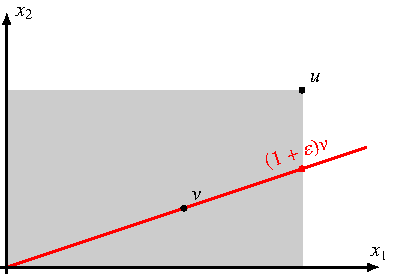
\includegraphics{chapters/80-wahrscheinlichkeit/images/trenn.pdf}
\caption{Die Vektoren $w\le u$ liegen im grauen Rechteck.
Zwei nichtnegative Vektoren $u$ und $v$ mit $u>v$
haben keine gleichen Komponenten.
Daher kann man $v$ mit einer Zahl $\vartheta=1+\varepsilon > 1$
strecken, so dass der gestreckte Vektor $(1+\varepsilon)v$ gerade noch
im grauen Rechteck liegt: $u\ge (1+\varepsilon)v$.
Streckung mit einem grösseren Faktor führt dagegen aus dem Rechteck
hinaus.
\label{buch:wahrscheinlichkeit:figure:trenn}}
\end{figure}

\begin{satz}[Trenntrick]
\label{buch:wahrscheinlichkeit:satz:trenntrick}
\index{Trenntrick}%
Sind $u$ und $v$ nichtnegative Vektoren und $u>v$, dann gibt es eine
positive Zahl $\varepsilon>0$ derart, dass
$u\ge (1+\varepsilon)v$.
Ausserdem kann $\varepsilon$ so gewählt werden, dass $u\not\ge(1+\mu)v$
für $\mu>\varepsilon$.
\end{satz}

\begin{proof}[Beweis]
Wir betrachten die Zahl
\[
\vartheta
=
\max_{v_i\ne 0} \frac{u_i}{v_i}.
\]
Wegen $u>v$ sind die Quotienten auf der rechten Seite alle $>1$.
Da nur endlich viele Quotienten miteinander verglichen werden, ist
daher auch $\vartheta >1$.
Es folgt $u\ge \vartheta v$. 
Wegen $\vartheta >1$ ist $\varepsilon = \vartheta -1 >0$ und
$u\ge (1+\varepsilon)v$.
\end{proof}

Der Satz besagt also, dass es eine Komponente $v_i\ne 0$ gibt
derart, dass $u_i = (1+\varepsilon)v_i$.
Diese Komponenten limitiert also, wie stark man $v$ strecken kann,
so dass er immer noch $\le u$ ist.
Natürlich folgt aus den der Voraussetzung $u>v$ auch, dass $u$ ein 
positiver Vektor ist (Abbildung~\ref{buch:wahrscheinlichkeit:figure:trenn}).

\begin{figure}
\centering
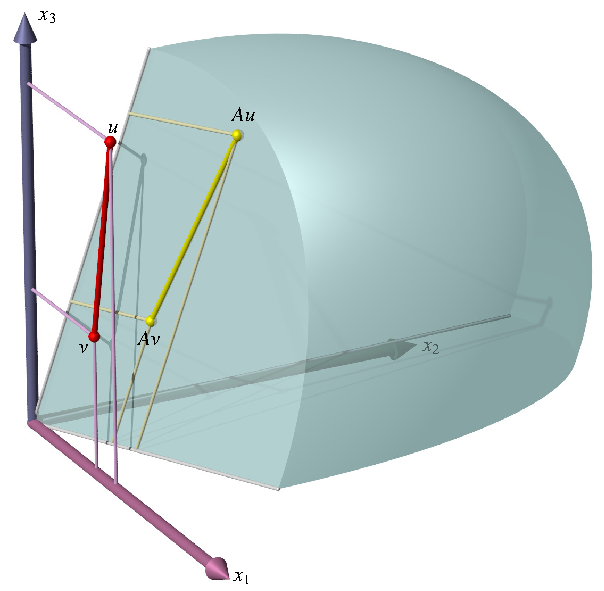
\includegraphics{chapters/80-wahrscheinlichkeit/images/vergleich.pdf}
\caption{Eine positive Matrix $A$ bildet nichtnegative Vektoren in
positive Vektoren ab
(Korollar~\ref{buch:wahrscheinlichkeit:satz:Au>0korollar}).
Zwei verschiedene Vektoren auf einer Seitenfläche erfüllen $u\ge v$,
aber nicht $u>v$, da sie sich in der Koordinaten $x_2$ nicht unterscheiden.
Die Bilder unter $A$ unterscheiden sich dann auch in $x_2$, es gilt
$Au>Av$ (siehe auch Satz~\ref{buch:wahrscheinlichkeit:satz:vergleichstrick})
\label{buch:wahrscheinlichkeit:fig:vergleich}}
\end{figure}

\begin{satz}[Vergleichstrick]
\label{buch:wahrscheinlichkeit:satz:vergleichstrick}
\index{Vergleichstrick}%
Sei $A$ eine positive Matrix und seinen $u$ und $v$ Vektoren
mit $u\ge v$ und $u\ne v$, dann ist $Au > Av$
(siehe auch Abbildung~\ref{buch:wahrscheinlichkeit:fig:vergleich}).
\end{satz}

\begin{proof}[Beweis]
Wir schreiben $d=u-v$, nach Voraussetzung ist $d\ne 0$.
Der Satz besagt dann, dass aus $d\ge 0$ folgt, dass $Ad>0$.
Dies müssen wir beweisen.

Die Ungleichung $Ad>0$ besagt, dass alle Komponenten von $Ad$ 
positiv sind.
Um dies nachzuweisen, berechnen wir
\begin{equation}
(Ad)_i
=
\sum_{j=1}^n
a_{i\!j}
d_j.
\label{buch:wahrscheinlichkeit:eqn:Adpositiv}
\end{equation}
Alle Koeffizienten  $a_{i\!j}$ sind $>0$, weil $A$ positiv ist.
Mindestens eine der Komponenten $d_j$ ist $>0$, weil $d\ne 0$.
Insbesondere sind alle Terme der Summe $\ge 0$, woraus wir
bereits schliessen können, dass $(Ad)_i\ge 0$ sein muss.
Die Komponente $d_j>0$ liefert einen positiven Beitrag
$a_{i\!j}d_j>0$
zur Summe~\eqref{buch:wahrscheinlichkeit:eqn:Adpositiv},
also ist $(Ad)_i>0$.
\end{proof}

Der folgende Spezialfall folgt unmittelbar aus dem
Satz~\ref{buch:wahrscheinlichkeit:satz:vergleichstrick}.

\begin{korollar}
\label{buch:wahrscheinlichkeit:satz:Au>0korollar}
Ist $A$ eine positive Matrix und $u\ge 0$ mit $u\ne 0$, dann
ist $Au>0$.
\end{korollar}

Eine positive Matrix macht also aus nicht verschwindenden,
nicht negativen Vektoren positive Vektoren.

%
% Die verallgemeinerte Dreiecksungleichung
%
\subsection{Die verallgemeinerte Dreiecksungleichung
\label{buch:subsection:verallgemeinerte-dreiecksungleichung}}
Die Dreiecksungleichung besagt, dass für beliebige Vektoren
$u,v\in\mathbb{R}^n$ gilt
\[
|u+v|\le |u|+|v|
\]
mit Gleichheit genau dann, wenn $u$ und $v$ linear abhängig sind.
Wenn beide von $0$ verschieden sind, dann gibt es eine positive Zahl
$t$ mit $u=tv$.
Wir brauchen eine Verallgemeinerung für eine grössere Zahl von
Summanden.

\begin{figure}
\centering
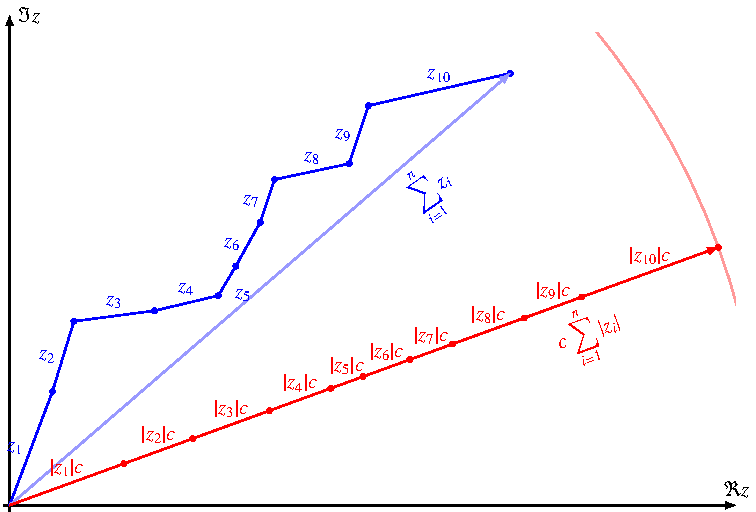
\includegraphics{chapters/80-wahrscheinlichkeit/images/dreieck.pdf}
\caption{Die verallgemeinerte Dreiecksungleichung von
Satz~\ref{buch:wahrscheinlichkeit:satz:verallgemeinerte-dreiecksungleichung}
besagt, dass
die Länge einer Summe von Vektoren (blau) höchstens so gross ist wie die
Summe der Längen, mit Gleichheit genau dann, wenn alle Vektoren die
gleiche Richtung haben (rot).
Hier dargestellt am Beispiel von Zahlen in der komplexen Zahlenebene.
In dieser Form wird die verallgemeinerte Dreiecksungleichung in
Satz~\ref{buch:wahrscheinlichkeit:satz:verallgdreieckC}
angewendet.
\label{buch:wahrscheinlichkeit:fig:dreieck}}
\end{figure}

\begin{satz}[Verallgemeinerte Dreiecksungleichung]
\label{buch:wahrscheinlichkeit:satz:verallgemeinerte-dreiecksungleichung}
Für $n$ Vektoren $v_i\ne 0$ gilt
\[
|u_1+\dots+u_n| \le |u_1|+\dots+|u_n|
\]
mit Gleichheit genau dann, wenn alle Vektoren nichtnegative Vielfache
eines gemeinsamen Einheitsvektors $c$ sind: $u_i=|u_i|c$
(siehe auch Abbildung~\ref{buch:wahrscheinlichkeit:fig:dreieck}).
\end{satz}

\begin{proof}[Beweis]
Die Aussage kann mit vollständiger Induktion bewiesen werden.
Die Induktionsverankerung ist der Fall $n=2$, gegeben durch die
gewöhnliche Dreiecksungleichung.

Wir nehmen daher jetzt an, die Aussage sei für $n$ bereits bewiesen,
wir müssen sie für $n+1$ beweisen.
Die Summe von $n+1$ Vektoren kann man in $u=u_1+\dots+u_n$ und $v=u_{n+1}$
aufteilen.
Es gilt nach der gewöhnlichen Dreiecksungleichung, dass
\[
|u+v|
=
|u_1+\dots+u_n+u_{n+1}|
\le
|u_1+\dots+u_n|+|u_{n+1}|
\]
mit Gleichheit genau dann, wenn $u_1+\dots+u_n$ und $u_{n+1}$
linear abhängig sind.
Nach Induktionsannahme gilt ausserdem
\[
|u_1+\dots+u_n| \le |u_1|+\dots+|u_n|
\]
mit Gleichheit genau dann, wenn die Vektoren $u_1,\dots,u_n$
positive Vielfache eines Einheitsvektors $u$ sind, $u_i=|u_i|c$.
Es ist dann
\[
u=u_1+\dots+u_n
=
\biggl(\sum_{i=1}^n |u_i|c\biggr)
=
\biggl(\sum_{i=1}^n |u_i|\biggr)c.
\]
Da $|u+v|=|u|+|v|$ genau dann gilt, wenn $u$ und $v$ linear abhängig sind,
folgt jetzt, dass $v$ ebenfalls ein nichtnegatives Vielfaches von $c$ ist.
Damit ist der Induktionsschritt vollzogen.
\end{proof}

\begin{satz}
\label{buch:wahrscheinlichkeit:satz:verallgdreieckC}
Seien $a_1,\dots,a_n$ positive Zahlen und $u_i\in\mathbb C$ derart,
dass 
\[
\biggl|
\sum_{i=1}^n a_i u_i
\biggr|
=
\sum_{i=1}^n a_i |u_i|,
\]
dann gibt es eine komplexe Zahl $c$ und einen nichtnegativen Vektor $v$
derart, dass $u=cv$.
\end{satz}

Der Satz besagt, dass die komplexen Komponenten $u_i$ alle das gleiche
Argument haben.
Die motiviert den nachstehenden geometrischen Beweis des Satzes.

\begin{proof}[Beweis]
Wer stellen uns die komplexen Zahlen $u_i$ als Vektoren in der
zweidimensionalen Gauss\-schen Ebene vor.
Dann ist die Aussage nichts anderes als ein Spezialfall von
Satz~\ref{buch:wahrscheinlichkeit:satz:verallgemeinerte-dreiecksungleichung}
für den zweidimensionalen reellen Vektorraum $\mathbb{C}$.
\end{proof}


%
% Der Satz von Perron-Frobenius
%
\subsection{Der Satz von Perron-Frobenius
\label{buch:subsection:der-satz-von-perron-frobenius}}
Wir sind an den Eigenwerten und Eigenvektoren einer positiven
oder primitiven Matrix interessiert.
Nach Definition des Spektralradius $\varrho(A)$ muss es einen Eigenvektor 
zu einem Eigenwert $\lambda$ mit Betrag $|\lambda|=\varrho(A)$ geben,
aber a priori wissen wir nicht, ob es einen reellen Eigenvektor zum
Eigenwert $\varrho(A)$ gibt.

\begin{figure}
\centering
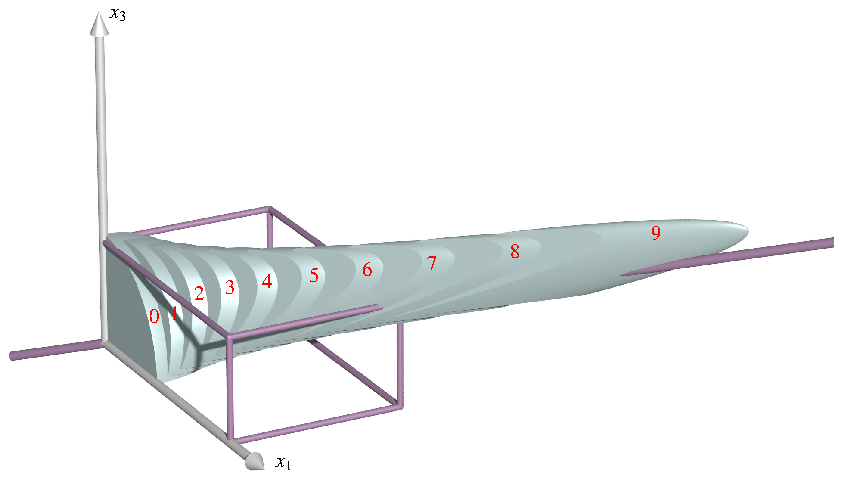
\includegraphics{chapters/80-wahrscheinlichkeit/images/positiv.pdf}
\caption{Die Iteration einer positiven Matrix bildet den positiven Oktanten
in immer enger werdende Kegel ab, die die Richtung des gesuchten Eigenvektors
gemeinsam haben.
\label{buch:wahrscheinlichkeit:figure:positiv}}
\end{figure}

In Abbildung~\ref{buch:wahrscheinlichkeit:fig:vergleich} kann man sehen,
dass eine positive Abbildung den positiven Oktanten in einen etwas engeren
Kegel hinein abbildet.
Iteriert man dies (Abbildung~\ref{buch:wahrscheinlichkeit:figure:positiv}),
wird die Bildmenge immer enger, bis sie nur ein
sehr enger Kegel um die Richtung des Eigenvektors ist.
Tatsächlich kann man aus dieser Idee auch einen topologischen
Beweis des untenstehenden Satzes von Perron-Frobenius konstruieren
(\cite{skript:pftopo} und
\cite{skript:hilbertmetric}).
Er beruht darauf, dass eine Abbildung, die Distanzen verkleinert,
einen Fixpunkt hat.
Die Konstruktion einer geeigneten Metrik ist allerdings eher 
kompliziert, weshalb wir im Beweise der nachstehenden Aussagen
den konventionellen Weg wählen.

Wir beginnen damit zu zeigen, dass für positive Matrizen $A$
nichtnegative Eigenvektoren zu Eigenwerten $\lambda\ne 0$
automatisch positiv sind.
Ausserdem müssen die zugehörigen Eigenwerte sogar positiv sein.

\begin{satz}
Sei $A$ eine positive Matrix und $u$ ein nichtnegativer Eigenvektor zum
Eigenwert $\lambda\ne 0$.
Dann ist $u$ ein positiver Vektor und $\lambda > 0$.
\end{satz}

\begin{proof}[Beweis]
Nach dem Korollar~\ref{buch:wahrscheinlichkeit:satz:Au>0korollar}
folgt, dass $Au>0$ ein positiver Vektor ist, es sind
also alle Komponenten positiv.
Der Vektor $u$ ist aber auch ein Eigenvektor, es gilt also
$\lambda u = Au$.
Da alle Komponenten von $Au$ positiv sind, müssen auch
alle Komponenten von $\lambda u$ positiv sein.
Das ist nur möglich, wenn $\lambda > 0$.
\end{proof}

Wenn $v$ ein Eigenvektor von $A$ ist, dann ist auch jedes Vielfache
davon ein Eigenvektor, insbesondere können einzelne Komponenten
des Vektors $v$ auch negativ sein.
Der folgende Satz zeigt aber, dass der Vektor aus den Beträgen
der Komponenten von $v$ ebenfalls ein Eigenvektor zum 
gleichen Eigenwert ist.
Insbesondere gibt es immer einen nichtnegativen Eigenvektor.

\begin{satz}
\label{buch:wahrscheinlichkeit:satz:positivereigenvektor}
Sei $A$ eine positive Matrix und $v$ ein Eigenvektor von $A$ zu einem
Eigenwert $\lambda$ mit Betrag $|\lambda|=\varrho(A)$,
dann ist der Vektor $u$  mit den Komponenten $u_i=|v_i|$ ein
positiver Eigenvektor zu Eigenwert $\varrho(A)$.
\end{satz}

\begin{proof}[Beweis]
Es gilt natürlich auch, dass
\[
(Au)_i
=
\sum_{j=1}^n a_{i\!j}u_j
=
\sum_{j=1}^n |a_{i\!j}v_j|
\ge
\biggl|
\sum_{j=1}^n a_{i\!j}v_j
\biggr|
=
|(Av)_i|
=
|\lambda v_i|
=
\varrho(A) |v_i|
=
\varrho(A) u_i,
\]
oder $Au \ge \varrho(A)u$.
Wir müssen zeigen, dass sogar $Au=\varrho(A)u$ gilt.
Wir nehmen daher an, dass $Au\ne \varrho(A)u$ ist, und führen dies zu
einem Widerspruch.

Da $\varrho(A)u$ ein nichtnegativer Vektor ist, können wir den Vergleichstrick
Satz~\ref{buch:wahrscheinlichkeit:satz:vergleichstrick}, auf die beiden
Vektoren $Au$ und $\varrho(A)u$ anwenden.
Wir schliessen $A^2u > \varrho(A)Au$.

Mit dem Trenntrick
Satz~\ref{buch:wahrscheinlichkeit:satz:trenntrick}
können wir jetzt eine Zahl $\vartheta>1$ finden derart, dass
\[
A^2 u \ge \vartheta \varrho(A) Au
\]
ist.
Durch wiederholte Anwendung von $A$ findet man
\begin{align}
A^3 u & \ge (\vartheta \varrho(A))^2 Au
\notag
\\
&\phantom{0}\vdots
\notag
\\
A^{k+1} u & \ge (\vartheta \varrho(A))^{k} Au
\label{buch:pf:eqn:ak+1}
\end{align}
Aus $|A^{k+1}u| \le \|A^k\|\,|Ak|$ und
\eqref{buch:pf:eqn:ak+1} kann man jetzt die Norm von $A^k$ abschätzen:
\[
\begin{aligned}
\| A^{k}\|\cdot |Au|
&\ge 
| A^{k+1}u|
\ge
(\vartheta\varrho(A))^{k}\, |Au|
&&
\Rightarrow
&
\|A^k\| &\ge  (\vartheta\varrho(A))^k 
\\
&&&\Rightarrow&
\|A^k\|^{\frac{1}{k}} &\ge \vartheta\varrho(A)
\\
&&&\Rightarrow&
\lim_{k\to\infty}
\|A^k\|^{\frac{1}{k}} &\ge \vartheta\varrho(A)
\\
&&&&\|\phantom{00}&
\\
&&&%\Rightarrow&
&
\varrho(A)&\ge \vartheta\varrho(A).
\end{aligned}
\]
Wegen $\vartheta>1$ ist dies aber gar nicht möglich.
Dieser Widerspruch zeigt, dass $u=v$ sein muss, insbesondere ist
$v$ ein nichtnegativer Eigenvektor.
\end{proof}

Die Potenzmethode funktioniert nur, wenn kein anderer Eigenwert
den Betrag $\varrho(A)$ hat.
Der folgende Satz garantiert dies.

\begin{satz}
Sei $A$ eine positive Matrix und $v$ ein Eigenvektor zu einem 
Eigenwert $\lambda$ mit Betrag $|\lambda|=\varrho(A)$.
Dann ist $\lambda=\varrho(A)$.
\end{satz}

\begin{proof}[Beweis]
Nach Satz~\ref{buch:wahrscheinlichkeit:satz:positivereigenvektor}
ist der Vektor $u$ mit den Komponenten $u_i=|v_i|$ ein positiver
Eigenvektor zum Eigenwert $\varrho(A)$.
Aus der Eigenvektorgleichung für $u$ folgt
\begin{equation}
Au = \varrho(A) u
\quad\Rightarrow\quad
\sum_{j=1}^n a_{i\!j}|v_j| = \varrho(A) |v_i|.
\label{buch:wahrscheinlichkeit:eqn:pev1}
\end{equation}
Anderseits ist $v$ ein Eigenvektor zum Eigenwert $\lambda$, also gilt
\[
\sum_{j=1}^n a_{i\!j}v_j = \lambda v_i.
\]
Der Betrag davon ist
\begin{equation}
\biggl|
\sum_{j=1}^n a_{i\!j}v_j
\biggr|
=
|\lambda v_i|
=
\varrho(A) |v_i|.
\label{buch:wahrscheinlichkeit:eqn:pev2}
\end{equation}
Die beiden Gleichungen
\eqref{buch:wahrscheinlichkeit:eqn:pev1}
und
\eqref{buch:wahrscheinlichkeit:eqn:pev2}
zusammen ergeben die Gleichung
\begin{equation}
\biggl|
\sum_{j=1}^n a_{i\!j}v_j
\biggr|
=
\sum_{j=1}^n a_{i\!j}|v_j|.
\label{buch:pf:eqn:gleich}
\end{equation}
Nach der verallgemeinerten Dreiecksungleichung
Satz~\ref{buch:subsection:verallgemeinerte-dreiecksungleichung}
folgt jetzt aus der Gleichheit in~\eqref{buch:pf:eqn:gleich},
dass es eine komplexe Zahl $c$ vom Betrag $1$ gibt derart,
dass $v_j = |v_j|c=u_jc$.
Insbesondere ist $v=cu$.
Damit kann man jetzt $\lambda$ berechnen, es ist
\[
\lambda v = Av = Acu = c Au = c\varrho(A) u = \varrho(A) v,
\]
woraus $\lambda=\varrho(A)$ folgt.
\end{proof}

In Anwendungen wollen wir schliessen, dass die Grenzverteilung
eindeutig ist, dazu ist notwendig, dass der Eigenraum des
Eigenwertes $\varrho(A)$ eindimensional ist.

\begin{satz}
\label{buch:wahrscheinlichkeit:satz:geometrischeinfach}
Der Eigenraum $E_{\varrho(A)}(A)$ einer positiven Matrix $A$
zum Eigenwert $\varrho(A)$ ist eindimensional.
\end{satz}

\begin{proof}[Beweis]
Sei $u$ der bereits gefundene Eigenvektor von $A$ zum Eigenwert $\varrho(A)$
und sei $v$ ein weiterer, linear unabhängiger Eigenvektor zum
gleichen Eigenwert.
Da $A$ und $\varrho(A)$ reell sind, sind auch die Vektoren $\Re v$ und $\Im v$
aus den Realteilen $\Re v_i$ oder den Imaginärteilen $\Im v_i$ Eigenvektoren.
Beide Vektoren sind reelle Vektoren und mindestens einer davon ist mit
$u$ linear unabhängig.
Wir dürfen daher annehmen, dass $v$ ein linear unabhängiger Eigenvektor
zum Eigenwert $\varrho(A)$ ist.

Weil wir wissen, dass $u$ ein positiver Vektor ist, gibt es einen
grösstmöglichen Faktor $c>0$ derart, dass $u\ge cv$ oder $u\ge cv$.
Insbesondere verschwindet mindestens eine Komponente von $u-cv$.
Da $u$ und $v$ Eigenvektoren zum Eigenwert $\varrho(A)$ sind,
ist 
\[
A(u-cv)
=
\varrho(A)(u-cv).
\]
Der Vektor auf der rechten Seite hat mindestens eine verschwindende 
Komponente.
Der Vektor auf der linken Seite ist nach dem Vergleichstrick
Satz~\ref{buch:wahrscheinlichkeit:satz:vergleichstrick}
\[
A(u-cv) > 0,
\]
alle seine Komponenten sind $>0$.
Dieser Widerspruch zeigt, dass die Annahme, es gäbe einen von $u$ linear 
unabhängigen Eigenvektor zum Eigenwert $\varrho(A)$ nicht haltbar ist.
\end{proof}

Satz~\ref{buch:wahrscheinlichkeit:satz:geometrischeinfach} garantiert,
dass der Eigenwert einfach ist.
Es ist aber immer noch möglich, dass die algebraische Vielfachheit
von $\varrho(A) >1$ ist, dass also $\dim\mathcal{E}_{\varrho(A)}(A)>1$
ist.
Dies ist jedoch nicht der Fall.

\begin{satz}
\label{buch:wahrscheinlichkeit:satz:algebraischeinfach}
Sei $A$ eine positive Matrix und $p^t$ ein positiver Eigenvektor
der Matrix $A^t$ zum Eigenwert $\varrho(A^t)=\varrho(A)$.
Ist $u$ der Eigenvektor von $A$ zum Eigenwert $\varrho(A)$ nach
Satz~\ref{buch:wahrscheinlichkeit:satz:geometrischeinfach},
dann ist
\[
\mathbb{R}^n
=
\langle u\rangle
\oplus
\{ x\in\mathbb{R}^n \mid px=0\}
=
\langle u\rangle
\oplus
\ker p
\]
eine Zerlegung in invariante Unterräume von $A$.
Insbesondere ist der verallgemeinerte Eigenraum $\mathcal{E}_{\varrho(A)}(A)$
von $A$ eindimensional.
\end{satz}

\begin{proof}[Beweis]
Die beiden Vektoren $x$ und $p$ sind beide positiv, daher ist das 
Produkt $pu\ne 0$.
Insbesondere ist $u\not\in\ker p$

Es ist klar, dass $A\langle u\rangle = \langle Au\rangle = \langle u\rangle$
ein invarianter Unterraum ist.
Für einen Vektor $x\in\mathbb{R}^n$ mit $px=0$, also $x\in\ker p$,
erfüllt das Bild $Ax$ die Gleichung
\[
p(Ax)=(pA)x=(A^tp^t)^tx=
\varrho(A)(p^t)^tx
=
\varrho(A)px = 0,
\]
somit ist $A\ker p \subset \ker p$.
Beide Räume sind also invariante Unteräume.

$\ker p$ ist $(n-1)$-dimensional, $\langle u\rangle$ ist eindimensional
und $u$ ist nicht in $\ker p$ enthalten.
Folglich spannen $\langle u\rangle$ und $\ker p$ den ganzen Raum auf.

Gäbe es einen weiteren linear unabhängigen Vektor im verallgemeinerten
Eigenraum $\mathcal{E}_{\varrho(A)}(A)$, dann müsste es auch einen
solchen Vektor in $\ker p$ geben.
Da $\ker p$ invariant ist, müsste es also auch einen weiteren Eigenvektor
$u_2$ zum Eigenwert $\varrho(A)$ in $\ker p$ geben.
Die beiden Vektoren $u$ und $u_1$ sind dann beide Eigenvektoren, was
nach Satz~\ref{buch:wahrscheinlichkeit:satz:geometrischeinfach}
nicht möglich ist.
\end{proof}

Die in den Sätzen
\ref{buch:wahrscheinlichkeit:satz:positivereigenvektor}
bis
\ref{buch:wahrscheinlichkeit:satz:algebraischeinfach}
gefundenen Resultate können wir folgt zusammengefasst werden:

\begin{satz}[Perron-Frobenius]
\label{buch:wahrscheinlichkeit:satz:perron-frobenius}
Sei $A$ eine positive Matrix mit Spektralradius $\varrho(A)$.
Dann gibt es einen positiven Eigenvektor zum Eigenwert $\varrho(A)$,
mit geometrischer und algebraischer Vielfachheit $1$.
\end{satz}

\begin{beispiel}
In der Google-Matrix mit freiem Willen
nach
\eqref{buch:wahrscheinlichkeit:eqn:google-matrix}
enthält den Term $((1-\alpha)/N)UU^t$.
Die Matrix $UU^t$ ist eine Matrix aus lauter Einsen, der Term
ist also für $\alpha < 1$ eine positive Matrix.
Die Google-Matrix ist daher eine positive Matrix.
Nach dem Satz von Perron-Frobenius ist die Grenzverteilung
eindeutig bestimmt.
\end{beispiel}

Der Satz~\ref{buch:wahrscheinlichkeit:satz:perron-frobenius}
von Perron-Frobenius kann auf primitive Matrizen verallgemeinert
werden.

\begin{satz}
\label{buch:wahrscheinlichkeit:satz:perron-frobenius2}
Sei $A$ ein primitive, nichtnegative Matrix.
Dann ist $\varrho(A)$ der einzige Eigenwert vom Betrag $\varrho(A)$
und er hat geometrische und algebraische Vielfachheit $1$.
\end{satz}

\begin{proof}[Beweisansatz]
Nach Voraussetzung gibt es ein $n$ derart, dass $A^n>0$.
Für $A^n$ gelten die Resultate von 
Satz~\ref{buch:wahrscheinlichkeit:satz:perron-frobenius}.
Man kann zeigen, dass die Eigenvektoren von $A^n$ auch 
Eigenvektoren von $A$ sind.
\end{proof}
